% Reflow the original figure into three rows. Pixel-exact crops preserve icons, code and data.
\begingroup
\definecolor{ch20teal}{RGB}{28,118,123}
\definecolor{ch20violet}{RGB}{153,99,240}
\definecolor{ch20flowbg}{RGB}{250,247,255}
\begin{tikzpicture}[x=0.0135514019cm,y=-0.0135514019cm,
  every node/.style={inner sep=0pt,outer sep=0pt,align=center,font=\sffamily\fontsize{10}{11.5}\selectfont}]
  \node[anchor=north west] at (0,0) {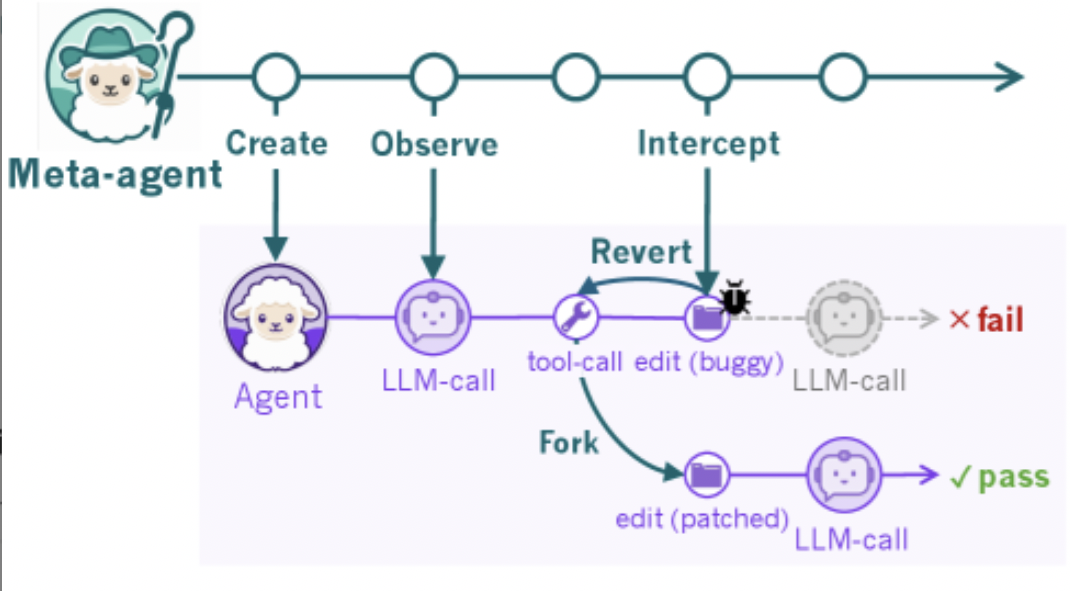
\includegraphics[width=14.5cm]{figures_zh/ch20/shepherd_flow.png}};
  \path[fill=white] (0,0) rectangle (3,591);
  \path[fill=white] (3,150) rectangle (226,205);
  \node[text=ch20teal,font=\sffamily\bfseries\fontsize{11}{12}\selectfont] at (111,175) {元智能体};
  \path[fill=white] (220,124) rectangle (334,160);
  \path[fill=white] (365,124) rectangle (507,160);
  \path[fill=white] (631,121) rectangle (789,166);
  \node[text=ch20teal,font=\sffamily\bfseries\fontsize{10}{11.5}\selectfont] at (278,143) {创建};
  \node[text=ch20teal,font=\sffamily\bfseries\fontsize{10}{11.5}\selectfont] at (435,143) {观测};
  \node[text=ch20teal,font=\sffamily\bfseries\fontsize{10}{11.5}\selectfont] at (709,143) {拦截};
  \path[fill=ch20flowbg] (229,376) rectangle (332,415);
  \node[text=ch20violet] at (280,396) {智能体};
  \path[fill=ch20flowbg] (587,233) rectangle (698,269);
  \node[text=ch20teal,font=\sffamily\bfseries\fontsize{10}{11.5}\selectfont] at (642,251) {回滚};
  \path[fill=ch20flowbg] (377,364) rectangle (505,398);
  \node[text=ch20violet,font=\sffamily\fontsize{9.5}{11}\selectfont] at (440,381) {LLM 调用};
  \path[fill=ch20flowbg] (521,347) rectangle (631,377);
  \node[text=ch20violet,font=\sffamily\fontsize{9}{10}\selectfont] at (576,362) {工具调用};
  \path[fill=ch20flowbg] (633,347) rectangle (791,377);
  \node[text=ch20violet,font=\sffamily\fontsize{8.5}{10}\selectfont] at (712,362) {编辑（有缺陷）};
  \path[fill=ch20flowbg] (792,364) rectangle (922,398);
  \node[text=gray,font=\sffamily\fontsize{9.5}{11}\selectfont] at (856,381) {LLM 调用};
  \path[fill=ch20flowbg] (975,300) rectangle (1057,339);
  \node[text=red!75!black,font=\sffamily\bfseries\fontsize{10}{11.5}\selectfont] at (1015,320) {失败};
  \path[fill=ch20flowbg] (530,427) rectangle (605,462);
  \node[text=ch20teal,font=\sffamily\bfseries\fontsize{9.5}{11}\selectfont] at (565,444) {派生分支};
  \path[fill=ch20flowbg] (612,504) rectangle (791,536);
  \node[text=ch20violet,font=\sffamily\fontsize{9}{10}\selectfont] at (704,519) {编辑（已修补）};
  \path[fill=ch20flowbg] (792,527) rectangle (923,558);
  \node[text=ch20violet,font=\sffamily\fontsize{9.5}{11}\selectfont] at (856,542) {LLM 调用};
  \path[fill=ch20flowbg] (976,459) rectangle (1062,500);
  \node[text=green!50!black,font=\sffamily\bfseries\fontsize{10}{11.5}\selectfont] at (1018,479) {通过};
\end{tikzpicture}
\par\vspace{2mm}
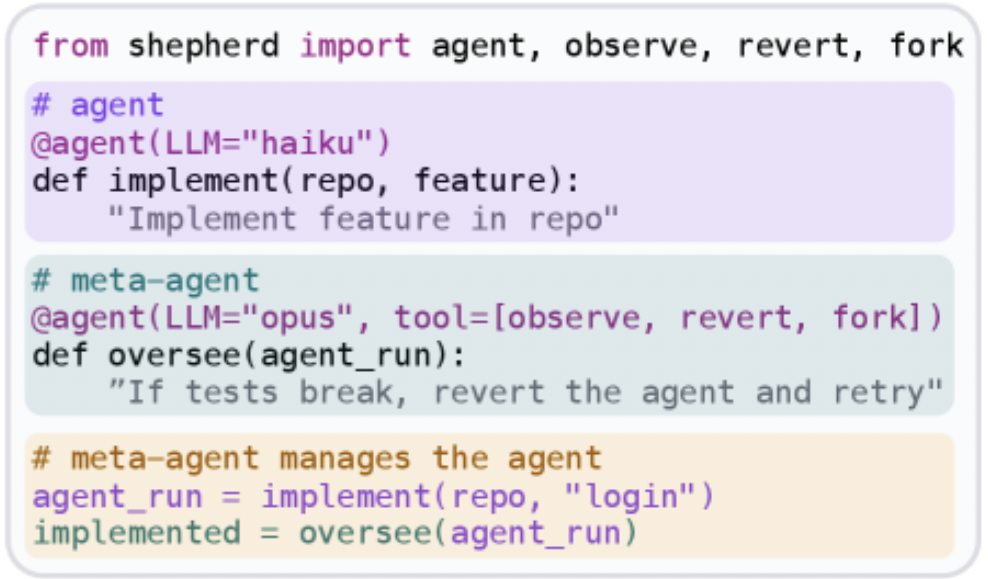
\includegraphics[width=12.5cm]{figures_zh/ch20/shepherd_code.png}
\par\vspace{2mm}
\begin{tikzpicture}[x=0.0075480769cm,y=-0.0075480769cm,
  every node/.style={inner sep=0pt,outer sep=0pt,align=center,font=\sffamily\fontsize{7.5}{8.5}\selectfont}]
  \node[anchor=north west] at (0,0) {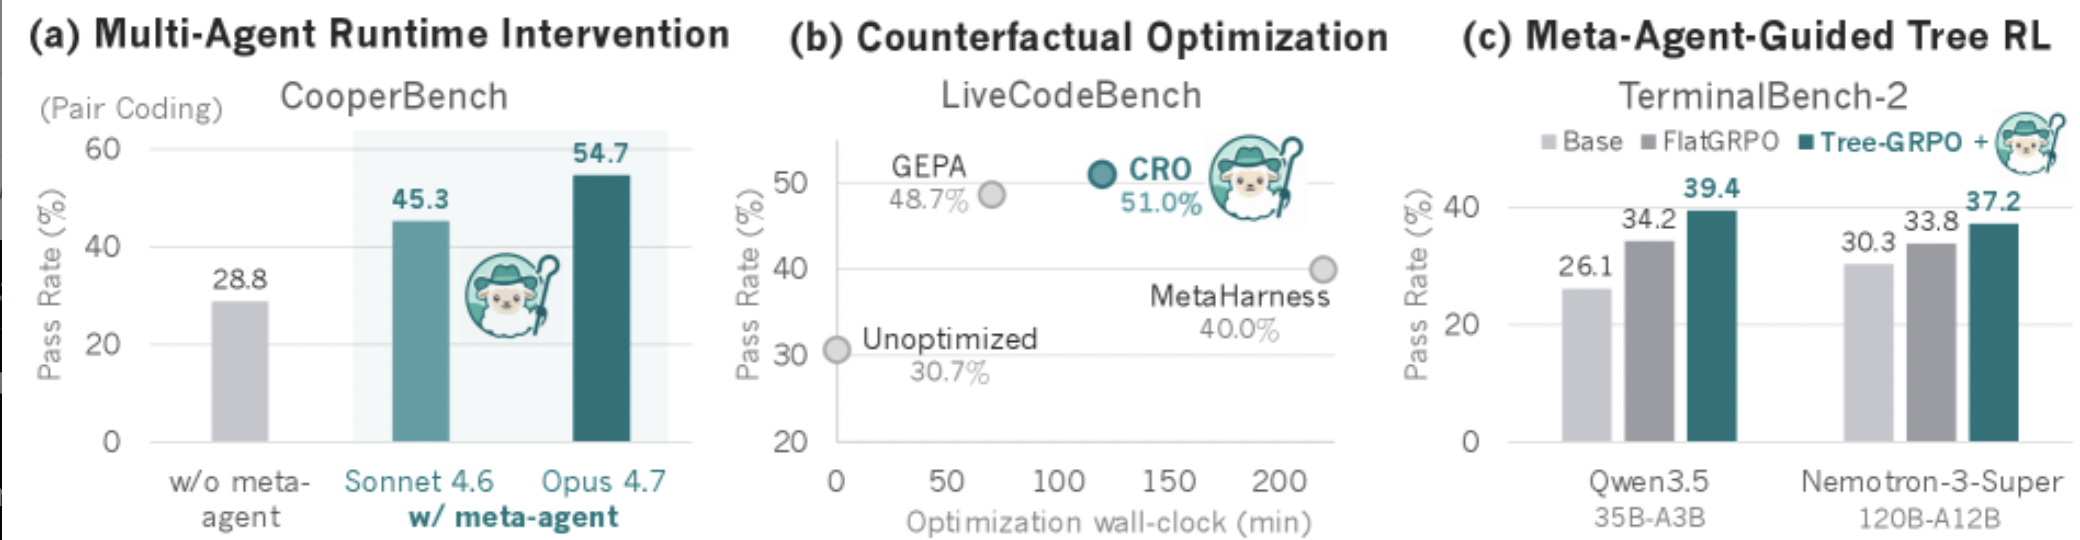
\includegraphics[width=15.7cm]{figures_zh/ch20/shepherd_charts.png}};
  \path[fill=white] (0,0) rectangle (3,540);
  \path[fill=white] (20,11) rectangle (742,60);
  \path[fill=white] (782,11) rectangle (1394,60);
  \path[fill=white] (1454,11) rectangle (2070,60);
  \node[font=\sffamily\bfseries\fontsize{8}{9}\selectfont] at (381,34) {(a) 多智能体运行时干预};
  \node[font=\sffamily\bfseries\fontsize{8}{9}\selectfont] at (1088,34) {(b) 反事实优化};
  \node[font=\sffamily\bfseries\fontsize{8}{9}\selectfont] at (1762,34) {(c) 元智能体引导的树式强化学习};
  \path[fill=white] (37,91) rectangle (230,126);
  \node at (133,109) {（结对编程）};
  \path[fill=white] (30,185) rectangle (69,384);
  \path[fill=white] (733,185) rectangle (771,384);
  \path[fill=white] (1398,185) rectangle (1437,384);
  \node[rotate=90] at (48,284) {通过率（\%）};
  \node[rotate=90] at (752,284) {通过率（\%）};
  \node[rotate=90] at (1410,284) {通过率（\%）};
  \path[fill=white] (164,465) rectangle (314,539);
  \node at (239,499) {无元智能体};
  \path[fill=white] (380,502) rectangle (666,539);
  \node[text=ch20teal,font=\sffamily\bfseries\fontsize{7.5}{8.5}\selectfont] at (523,520) {使用元智能体};
  \path[fill=white] (860,318) rectangle (1067,357);
  \draw[draw={rgb,255:red,235;green,235;blue,235},line width=0.3pt] (860,350) -- (1067,350);
  \node at (961,331) {未优化};
  \path[fill=white] (887,506) rectangle (1329,540);
  \node at (1108,523) {优化实际耗时（分钟）};
  \path[fill=white] (1560,126) rectangle (1626,158);
  \node at (1593,142) {基础};
\end{tikzpicture}
\endgroup
